%%%%%%%%%%%%%%%%%%%%%%%%%%%%%%%%%%%%%%%%%%%%%%%%%%%%%%%%%%%%%%%%%%%%%%
%%  Copyright by Wenliang Du.                                       %%
%%  This work is licensed under the Creative Commons                %%
%%  Attribution-NonCommercial-ShareAlike 4.0 International License. %%
%%  To view a copy of this license, visit                           %%
%%  http://creativecommons.org/licenses/by-nc-sa/4.0/.              %%
%%%%%%%%%%%%%%%%%%%%%%%%%%%%%%%%%%%%%%%%%%%%%%%%%%%%%%%%%%%%%%%%%%%%%%

\newcommand{\commonfolder}{../../common-files}
\newcommand{\webcommon}{../Web_Common}

\documentclass[11pt]{article}

\usepackage[most]{tcolorbox}
\usepackage{times}
\usepackage{epsf}
\usepackage{epsfig}
\usepackage{amsmath, alltt, amssymb, xspace}
\usepackage{wrapfig}
\usepackage{fancyhdr}
\usepackage{url}
\usepackage{verbatim}
\usepackage{fancyvrb}
\usepackage{adjustbox}
\usepackage{listings}
\usepackage{color}
\usepackage{subfigure}
\usepackage{cite}
\usepackage{sidecap}
\usepackage{pifont}
\usepackage{mdframed}
\usepackage{textcomp}
\usepackage{enumitem}
\usepackage{ctex}


% Horizontal alignment
\topmargin      -0.50in  % distance to headers
\oddsidemargin  0.0in
\evensidemargin 0.0in
\textwidth      6.5in
\textheight     8.9in 

\newcommand{\todo}[1]{
\vspace{0.1in}
\fbox{\parbox{6in}{TODO: #1}}
\vspace{0.1in}
}


\newcommand{\unix}{{\tt Unix}\xspace}
\newcommand{\linux}{{\tt Linux}\xspace}
\newcommand{\minix}{{\tt Minix}\xspace}
\newcommand{\ubuntu}{{\tt Ubuntu}\xspace}
\newcommand{\setuid}{{\tt Set-UID}\xspace}
\newcommand{\openssl} {\texttt{openssl}}


\pagestyle{fancy}
\lhead{\bfseries SEED Labs}
\chead{}
\rhead{\small \thepage}
\lfoot{}
\cfoot{}
\rfoot{}


\definecolor{dkgreen}{rgb}{0,0.6,0}
\definecolor{gray}{rgb}{0.5,0.5,0.5}
\definecolor{mauve}{rgb}{0.58,0,0.82}
\definecolor{lightgray}{gray}{0.90}


\lstset{%
  frame=none,
  language=,
  backgroundcolor=\color{lightgray},
  aboveskip=3mm,
  belowskip=3mm,
  showstringspaces=false,
%  columns=flexible,
  basicstyle={\small\ttfamily},
  numbers=none,
  numberstyle=\tiny\color{gray},
  keywordstyle=\color{blue},
  commentstyle=\color{dkgreen},
  stringstyle=\color{mauve},
  breaklines=true,
  breakatwhitespace=true,
  tabsize=3,
  columns=fullflexible,
  keepspaces=true,
  escapeinside={(*@}{@*)}
}

\newcommand{\newnote}[1]{
\vspace{0.1in}
\noindent
\fbox{\parbox{1.0\textwidth}{\textbf{Note:} #1}}
%\vspace{0.1in}
}


%% Submission
\newcommand{\seedsubmission}{You need to submit a detailed lab report, with screenshots,
to describe what you have done and what you have observed.
You also need to provide explanation
to the observations that are interesting or surprising.
Please also list the important code snippets followed by
explanation. Simply attaching code without any explanation will not
receive credits.}

%% Book
\newcommand{\seedbook}{\textit{Computer \& Internet Security: A Hands-on Approach}, 2nd
Edition, by Wenliang Du. See details at \url{https://www.handsonsecurity.net}.}

%% Videos
\newcommand{\seedisvideo}{\textit{Internet Security: A Hands-on Approach},
by Wenliang Du. See details at \url{https://www.handsonsecurity.net/video.html}.}

\newcommand{\seedcsvideo}{\textit{Computer Security: A Hands-on Approach},
by Wenliang Du. See details at \url{https://www.handsonsecurity.net/video.html}.}

%% Lab Environment
\newcommand{\seedenvironment}{This lab has been tested on our pre-built
Ubuntu 16.04 VM, which can be downloaded from the SEED website.}






\newcommand{\seedlabcopyright}[1]{
\vspace{0.1in}
\fbox{\parbox{6in}{\small Copyright \copyright\ {#1}\ \ by Wenliang Du.\\
      This work is licensed under a Creative Commons
      Attribution-NonCommercial-ShareAlike 4.0 International License.
      If you remix, transform, or build upon the material, 
      this copyright notice must be left intact, or reproduced in a way that is reasonable to
      the medium in which the work is being re-published.}}
\vspace{0.1in}
}






\newcommand{\ubuntutwo}{{\tt Ubuntu12.04}\xspace}
\newcommand{\ubuntusix}{{\tt Ubuntu16.04}\xspace}


\lhead{\bfseries SEED Labs -- MD5 碰撞攻击实验}

\def \code#1 {\fbox{\scriptsize{\texttt{#1}}}}

\begin{document}


\newcommand{\mdFigs}{./Figs}

\begin{center}
{\LARGE MD5 碰撞攻击实验}
\end{center}

\seedlabcopyright{2018}




% *******************************************
% SECTION
% *******************************************
\section{绪论}


一个安全的单向哈希函数需要满足两个性质:单向性和抗碰撞性。
单向性确保给定一个哈希值 \texttt{h} ,
要找到一个输入 $M$ 使得 \texttt{hash($M$) = h} 是计算上不可行的。
抗碰撞性确保找出两个不同的输入 \texttt{$M_1$} 和 \texttt{$M_2$},
使得 \texttt{hash($M_1$) = hash($M_2$)} 是计算上不可行的。


有一些广泛使用的单向哈希函数在抗碰撞性上存在问题。
在 CRYPTO 2004 的最后一场会议上,王小云及其合作者
展示了针对 MD5 \cite{Black:2006:MD5} 的碰撞攻击。
2017 年 2 月, CWI Amsterdam 和 Google Research 宣布了
\textit{SHAttered} \index{SHAttered} 攻击可以破坏 SHA-1 \cite{shattered}的抗碰撞性。
尽管许多学生对于理解单向性的重要性没有什么困难,
但是理解为什么需要抗碰撞属性以及这些攻击会造成什么影响不是很容易。


该实验的学习目标是让学生真正了解碰撞攻击的影响,
并亲眼看到如果广泛使用的单向哈希函数的抗碰撞性被破坏会造成什么损害。
为了实现此目标,学生需要针对 MD5 哈希函数发起真实的的碰撞攻击。
使用这些攻击,学生应该能够创建有相同 MD5 哈希值但行为完全不同的两个程序。
本实验涵盖了以下几个话题:

\begin{itemize}[noitemsep]
\item 单向哈希函数, MD5
\item 抗碰撞性
\item 碰撞攻击
\end{itemize}


\paragraph{阅读材料}
关于单向哈希函数的介绍可以参见:

\begin{itemize}
\item Chapter 22 of the SEED Book, \seedbook
\end{itemize}



\paragraph{实验环境} \seedenvironmentB \ \
本实验使用了一个 Marc Stevens 编写的 ``Fast MD5 Collision Generation'' 工具。
在我们的虚拟机中,它的二进制文件的名字是 \texttt{md5collgen} ,
已经被安装在 \texttt{/usr/bin} 文件夹里。
如果你想把它安装到你自己的机器上,可以直接从 \url{https://www.win.tue.nl/hashclash/}
下载源代码。


%\paragraph{Reading Materials.} One-way hash function, its properties,
%applications, and attacks (including the one covered in this lab)
%are explained in great details in Chapter 18 of the
%book \textit{Computer Security: A Hands-on Approach}, written by Wenliang
%Du.

\paragraph{致谢} 本实验是在锡拉丘兹大学
电气工程与计算机科学系研究生 Vishtasp Jokhi 的帮助下开发的。

%\newpage


% *******************************************
% SECTION
% *******************************************
\section{实验任务}


% -------------------------------------------
% SUBSECTION
% -------------------------------------------
\subsection{任务 1: 生成两个有相同 MD5 哈希的不同文件}


在此任务中,我们将生成两个具有相同 MD5 哈希值的不同文件。
这两个文件的开头部分是相同的,即它们有相同前缀。
我们可以使用 \texttt{md5collgen} 程序来实现此目的,该程序允许我们提供具有任意内容的前缀文件。
图 \ref{md5:fig:md5collgen} 中说明了程序的工作方式。
以下命令为给定的前缀文件 \texttt{prefix.txt} 生成两个输出文件
\texttt{out1.bin} 和 \texttt{out2.bin}:

\begin{lstlisting}
$ md5collgen -p prefix.txt -o out1.bin out2.bin
\end{lstlisting}


\begin{figure}[htb]
	\centering
	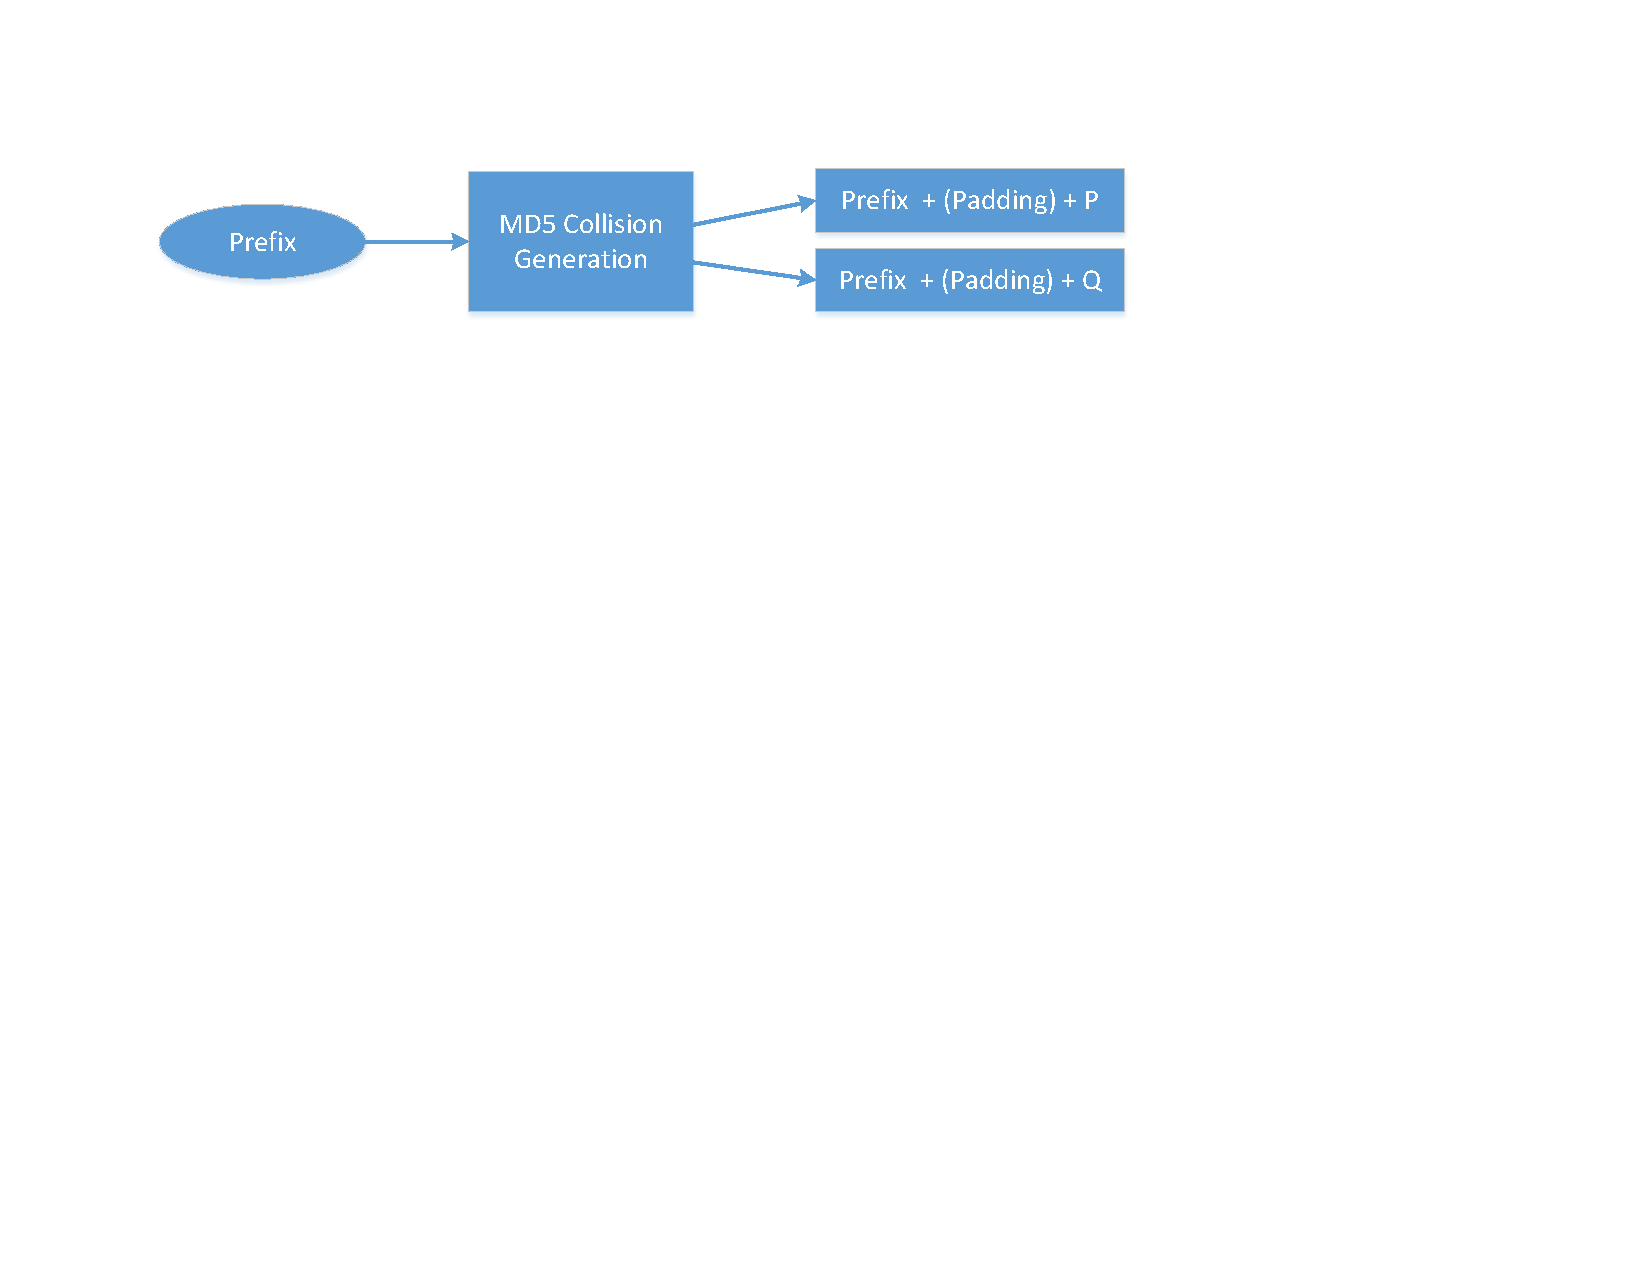
\includegraphics[width=0.8\textwidth]{\mdFigs/generate_collision.pdf}
	\caption{从一个前缀中生成 MD5 碰撞}
	\label{md5:fig:md5collgen}
\end{figure}


我们可以使用 \texttt{diff} 命令检查输出文件是否不同,
还可以使用 \texttt{md5sum} 命令来检查每个输出文件的 MD5 哈希值。
请参考以下命令。

\begin{lstlisting}
$ diff out1.bin out2.bin
$ md5sum out1.bin
$ md5sum out2.bin
\end{lstlisting}

由于 \texttt{out1.bin} 和 \texttt{out2.bin} 都是二进制文件,
我们不能使用文本查看程序( 例如 \texttt{cat} 或 \texttt{more} )查看它们。
我们需要使用一个二进制编辑器来查看(和编辑)它们。
我们已经在虚拟机中安装了一个名为 \texttt{bless} 的十六进制编辑器。
请使用这样的编辑器查看这两个输出文件,并描述你观察到的现象。
另外,你还应该回答下面的问题:


\begin{itemize}[label={--}]
  \item \textbf{问题 1.}
        如果前缀文件的长度不是 64 的倍数,会发生什么?

  \item \textbf{问题 2.}
        创建一个恰好有 64 个字节的前缀文件,再次运行碰撞工具,看看会发生什么?

  \item \textbf{问题 3.}
        在这两个文件中, \texttt{md5collgen} 生成的 128 字节数据是完全不同的吗?
        请找出所有不同的字节。
\end{itemize}


%If the same hash is generated by the above two commands, the program was successful and an MD5
%collision was generated.  If we use a hex editor to view the two output files generated
%previously, we can see that the beginning of both the files have the same prefix as specified
%in the prefix file. They also have 128 bytes of data which is appended to the prefix. The 128
%bytes of binary data added to each file is different for both files, and this is the part
%generated by the program which produces the MD5 collision.




% -------------------------------------------
% SUBSECTION
% -------------------------------------------
\subsection{任务 2: 理解 MD5 的性质}


在此任务中,我们将尝试了解 MD5 算法的一些性质。
这些性质对于我们在此实验中完成其他任务很重要。
MD5是一个非常复杂的算法,但是从高层次来看,它并不是那么复杂。
如图 \ref{md5:fig:how_md5_works} 所示, MD5 将输入数据划分为 64 个字节的块,
然后在这些块上迭代计算哈希。
MD5 算法的核心是压缩函数,该函数需要两个输入,即一个 64 字节的数据块和上一次迭代的结果。
压缩函数产生一个 128 位的 IHV ,代表 ``中间哈希值'' ; 然后将此输出馈入下一个迭代。
如果当前迭代是最后一次,则 IHV 将是最终的哈希值。
第一次迭代的 IHV 输入(IHV$_0$)是固定值。


\begin{figure}[htb]
	\centering
	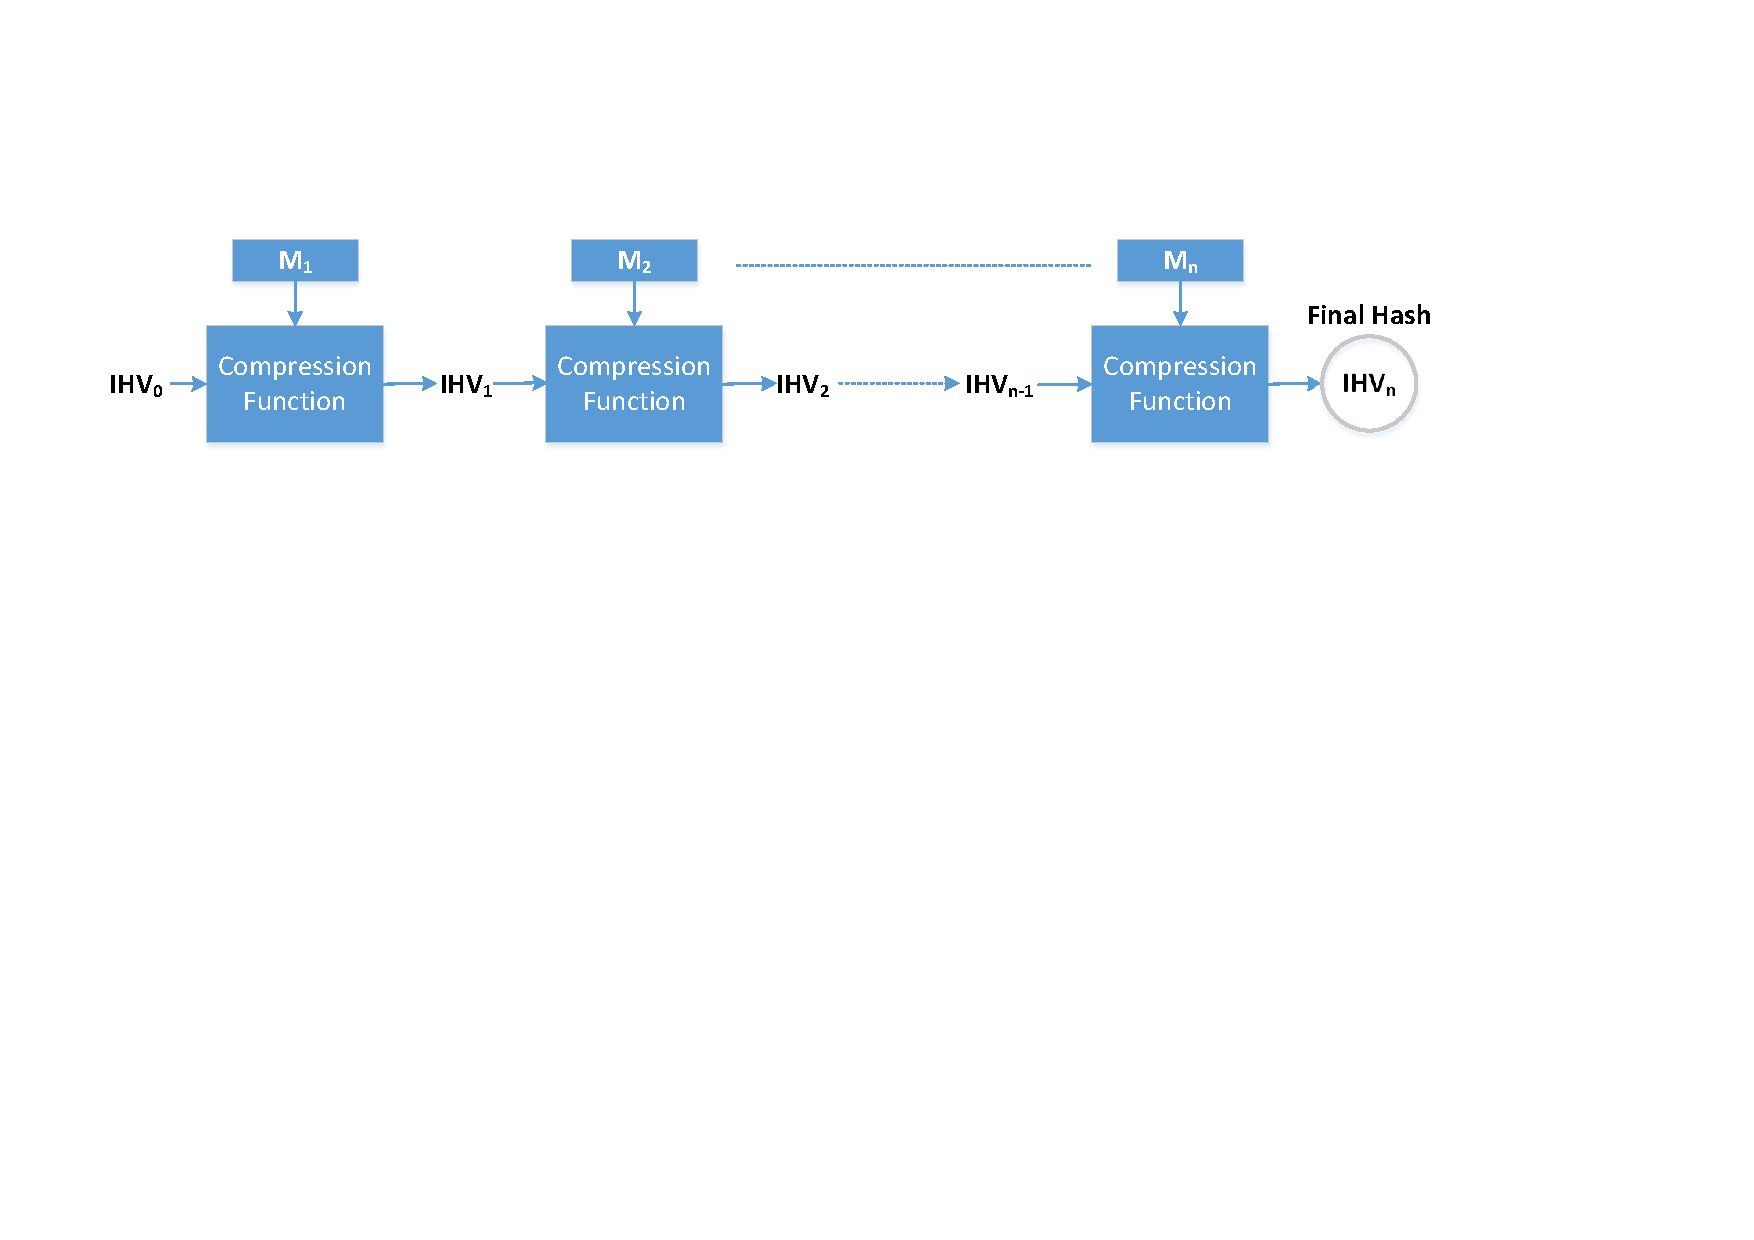
\includegraphics[width=0.90\textwidth]{\mdFigs/How_MD5_works.pdf}
	\caption{MD5 算法是怎样工作的}
	\label{md5:fig:how_md5_works}
\end{figure}


基于 MD5 的工作方式,我们可以得出 MD5 的下列性质:
给定两个输入 \texttt{M} 和 \texttt{N},如果 \texttt{MD5(M) = MD5(N)},
即 \texttt{M} 和 \texttt{N} 的 MD5 哈希是相同的,
那么对于任意的输入 \texttt{T}, \texttt{MD5(M $\|$ T) = MD5(N $\|$ T)},
这里 \texttt{$\|$} 表示连接。

也就是说,如果输入 \texttt{M} 和 \texttt{N} 有相同的哈希,
那么添加一个相同的后缀 \texttt{T} 就会得到两个有相同哈希值的输出。
这个性质不仅对 MD5 哈希算法成立,也对许多其他哈希算法成立。
\underline{你在本任务中的工作} 是要设计一个实验来说明这个性质对 MD5 成立。


你可以使用 \texttt{cat} 命令来将两个文件(无论是二进制文件还是文本文件)连接成一个。
下面的命令将 \texttt{file1} 和 \texttt{file2} 的内容连接起来,
将结果放到 \texttt{file3} 里。


\begin{lstlisting}
$ cat file1 file2 > file3
\end{lstlisting}



%\paragraph{Question 4.} With the understanding of how hash algorithms work (see
%Figure~\ref{md5:fig:how_md5_works}), we can now understand why the
%keyed hash used for MAC (Message Authenticating Code) does not simply calculate
%\texttt{hash(K $\|$ M)}, where \texttt{K} is the secret key, instead of using
%a more complicated HMAC algorithm. Please explain why it is not safe to
%simply use \texttt{hash(K $\|$ M)} to generate the MAC for message \texttt{M}.
%What attacks can you launch if this algorithm is used?
%Would you be able to launch the same attack if we swap the positions of \texttt{K}
%and \texttt{M}, i.e., the algorithm becomes \texttt{hash(M $\|$ K)}?



% -------------------------------------------
% SUBSECTION
% -------------------------------------------
\subsection{任务 3: 生成两个有相同 MD5 哈希的可执行文件}

在此任务中,我们提供了下面的 C 程序。
你的任务是创建该程序的两个不同版本,使 \texttt{xyz} 数组的内容不同,
但是可执行文件的哈希是相同的。


\begin{lstlisting}
#include <stdio.h>

unsigned char xyz[200] = {
 /* The actual contents of this array are up to you */
};

int main()
{
  int i;
  for (i=0; i<200; i++){
    printf("%x", xyz[i]);
  }
  printf("\n");
}
\end{lstlisting}


你可以选择在源代码层面完成这项工作,也就是上面的 C 程序的生成两个版本,
使得在编译后,它们对应的可执行文件有相同的 MD5 哈希值。
但是直接在二进制水平操作可能更加简单。
你可以在 \texttt{xyz} 数组中放任意的一些数,
然后你可以用一个十六进制编辑器来直接在二进制文件中修改 \texttt{xyz} 的内容。
找出这个数组存放在二进制文件中的哪个部分并不容易。
然而,如果我们在数组中填入一些固定的值,我们就能容易地在二进制文件中找到它们。
例如,下面的代码中数组被填满了 \texttt{0x41} , 即字母 \texttt{A} 的 ASCII 数值。
在二进制文件中找到 200 个 \texttt{A} 的位置不会很难。

\begin{lstlisting}
unsigned char xyz[200] = {
  0x41, 0x41, 0x41, 0x41, 0x41, 0x41, 0x41, 0x41, 0x41, 0x41,
  0x41, 0x41, 0x41, 0x41, 0x41, 0x41, 0x41, 0x41, 0x41, 0x41,
  0x41, 0x41, 0x41, 0x41, 0x41, 0x41, 0x41, 0x41, 0x41, 0x41,
  ... (omitted) ...
  0x41, 0x41, 0x41, 0x41, 0x41, 0x41, 0x41, 0x41, 0x41, 0x41,
}
\end{lstlisting}


\paragraph{实验指导}
在数组内部,我们可以找到两个位置将可执行文件分为三个部分:前缀、 128 字节区域和后缀。
前缀的长度必须是 64 个字节的倍数。
有关如何分割文件的说明,请参见图 \ref{md5:fig:fill_array}。

\begin{figure}[htb]
\centering
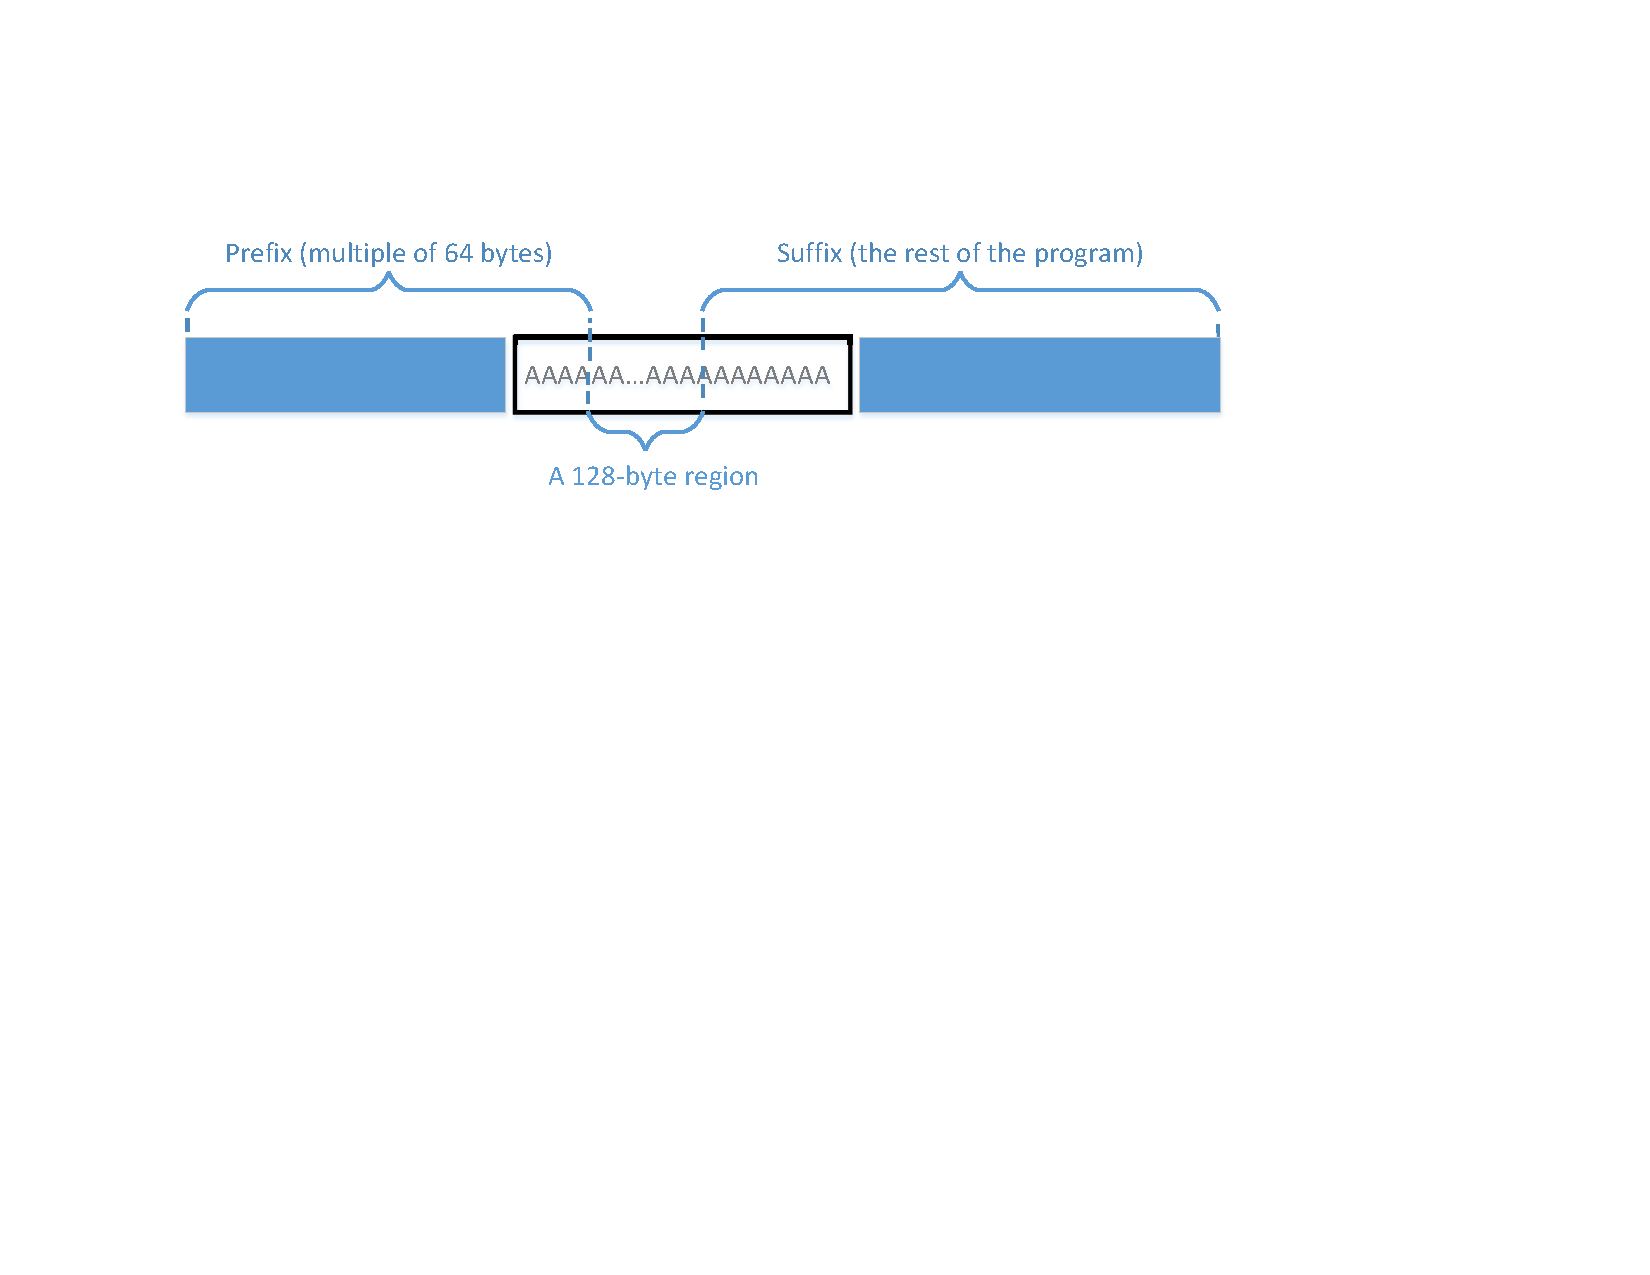
\includegraphics[width=0.9\textwidth]{\mdFigs/fill_array.pdf}
\caption{把可执行文件分成三个部分}
\label{md5:fig:fill_array}
\end{figure}

我们可以在前缀上运行 \texttt{md5collgen} 生成两个有相同 MD5 哈希值的输出。
让我们用 \texttt{P} 和 \texttt{Q} 来表示这些输出的第二个部分(即前缀之后,128 字节的部分)。
这样我们就有下面的条件:

\begin{lstlisting}
MD5 (prefix (*@$\|$@*) P) = MD5 (prefix (*@$\|$@*) Q)
\end{lstlisting}

根据 MD5 的性质,我们知道,如果将相同的后缀附加到上述两个输出中,得到的结果也将具有相同的哈希值。
下面的结论适用于所有后缀:

\begin{lstlisting}
MD5 (prefix (*@$\|$@*) P (*@$\|$@*) suffix) = MD5 (prefix (*@$\|$@*) Q (*@$\|$@*) suffix)
\end{lstlisting}

因此,我们只需要使用 \texttt{P} 和 \texttt{Q} 替换数组中两个分隔点之间的 128 个字节,
然后我们就可以创建两个有相同哈希值的二进制文件。
这两个程序的结果是不同的,因为它们分别输出它们自己的数组,而数组有不同的内容。


\paragraph{工具} 你可以使用 \texttt{bless} 来查看二进制可执行文件,找到数组的位置。
我们有一些工具可以用来在特定的位置分割一个二进制文件。
\texttt{head} 和 \texttt{tail} 命令都是很有用的工具。
你可以查看手册来了解如何使用它们。
我们在下面给出三个示例:

\begin{lstlisting}
$ head -c 3200 a.out > prefix
$ tail -c 100 a.out > suffix
$ tail -c +3300 a.out > suffix
\end{lstlisting}

第一个命令把 \texttt{a.out} 的前 \texttt{3200} 个字节保存到 \texttt{prefix} 文件中。
第二个命令把 \texttt{a.out} 的最后 \texttt{100} 个字节保存到 \texttt{suffix} 文件中。
第三个命令把 \texttt{a.out} 的最后 \texttt{100} 个字节保存到 \texttt{suffix} 文件中。
第三个命令把 \texttt{a.out} 从第 \texttt{3300} 个字节到末尾保存到 \texttt{suffix} 中。
使用这两个命令,我们可以从任意位置将一个二进制文件分割成几份。
如果我们需要把这几部分粘起来,我们可以使用 \texttt{cat} 命令。


如果你使用 \texttt{bless} 从一个二进制文件复制粘贴一块数据到另一个文件,
菜单中的 \texttt{"Edit -> Select Range"} 非常的好用,
因为你可以使用起始位置和范围来选择一块数据,而不需要手动数有多少数据被选中了。




% -------------------------------------------
% SUBSECTION
% -------------------------------------------
\subsection{任务 4: 是两个程序有不同的行为}


在上一个任务中,我们成功创建了两个具有相同 MD5 哈希值的程序,但是它们的行为不同。
但是,它们的区别仅在于它们打印出的数据。
他们仍然执行相同的指令序列。
在此任务中,我们希望做一些更明显且有意义的事。

假设你已经创建了一个做好事的软件。
你将软件发送给受信任的机构进行认证。
该机构对你的软件进行了全面的测试,并得出结论,你的软件确实在做好事。
权威机构将向你提供证书,说明你的程序是好的。
为了防止你在获得证书后更改程序,证书中还包括了程序的 MD5 哈希值;
证书是由权威机构签名的,因此你在不使签名无效的情况下不能更改证书或程序上的任何内容。


您想让您的恶意软件获得授权机构的认证,但是如果您只是将恶意软件发送给授权机构,
则不太可能实现该目标。
但是,你已经注意到,授权机构使用 MD5 生成哈希值。
你有个想法,你计划准备两个不同的程序。
一个程序将始终执行正常指令做好事,而另一个程序将执行恶意指令并造成损害。
你找到一种使这两个程序有相同 MD5 哈希值的方法。

然后,你将正常的版本发送给认证机构。
由于此版本只做正常的操作,它将通过认证,并且你将获得一个包含程序的哈希值的证书。
由于你的恶意程序具有相同的哈希值,因此该证书也对你的恶意程序有效。
这样,你已成功获取恶意程序的有效证书。
如果其他人信任颁发机构颁发的证书,他们将下载你的恶意程序。

\underline{此任务的目标} 是要发起上面描述这种攻击。
即,你需要创建两个有相同 MD5 哈希值的程序。
但是,一个程序将始终执行正常指令,而另一个程序将执行恶意指令。
在你的工作中,执行什么指令并不重要;只要证明这两个程序执行的指令是不同的就足够了。



\paragraph{实验指导}
创建两个有相同 MD5 哈希值且完全不同的程序非常困难。
\texttt{md5collgen} 生成的两个有相同哈希的程序需要共享相同的前缀;
此外,从上一个任务可以看出,如果我们需要在 \texttt{md5collgen} 产生的输出中添加一些
有意义的后缀,则添加到两个程序中的后缀也必须相同。
这些是我们使用的 MD5 碰撞生成程序的局限性。
尽管还有其他更复杂,更高级的工具可以克服某些限制,例如接受两个不同的前缀 \cite{stevens2007},
但它们需要更多的算力,因此不在本实验的范围之内。
我们需要找到一种方法来在有限的范围内生成两个不同的程序。

有多种方法可以实现上述目标。
我们提供一种方法作为参考,但鼓励学生提出自己的想法。
教师可以考虑给学生自己的想法一些奖励。
在我们的方法中,我们创建两个数组 \texttt{X} 和 \texttt{Y}。
我们比较这两个数组的内容。
如果相同,则执行正常代码。
否则,执行恶意代码。请参见以下伪代码:


\begin{lstlisting}
Array X;
Array Y;

main()
{
  if(X's contents and Y's contents are the same)
      run benign code;
  else
      run malicious code;
  return;
}
\end{lstlisting}


我们可以使用一些值来初始化数组 \texttt{X} 和 \texttt{Y} ,
这些值可以帮助我们在二进制可执行文件中找到它们的位置。
我们的工作是更改这两个数组的内容,这样我们可以生成具有相同 MD5 哈希值的两个不同版本。
在一个版本中, X 和 Y 的内容相同,因此执行正常代码。
在另一个版本中, X 和 Y 的内容不同,因此将执行恶意代码。
我们可以使用类似于任务 3 中使用的技术来实现此目标。
图 \ref{md5:fig:two_versions} 展示了程序的两个版本的区别。

\begin{figure}[htb]
	\centering
	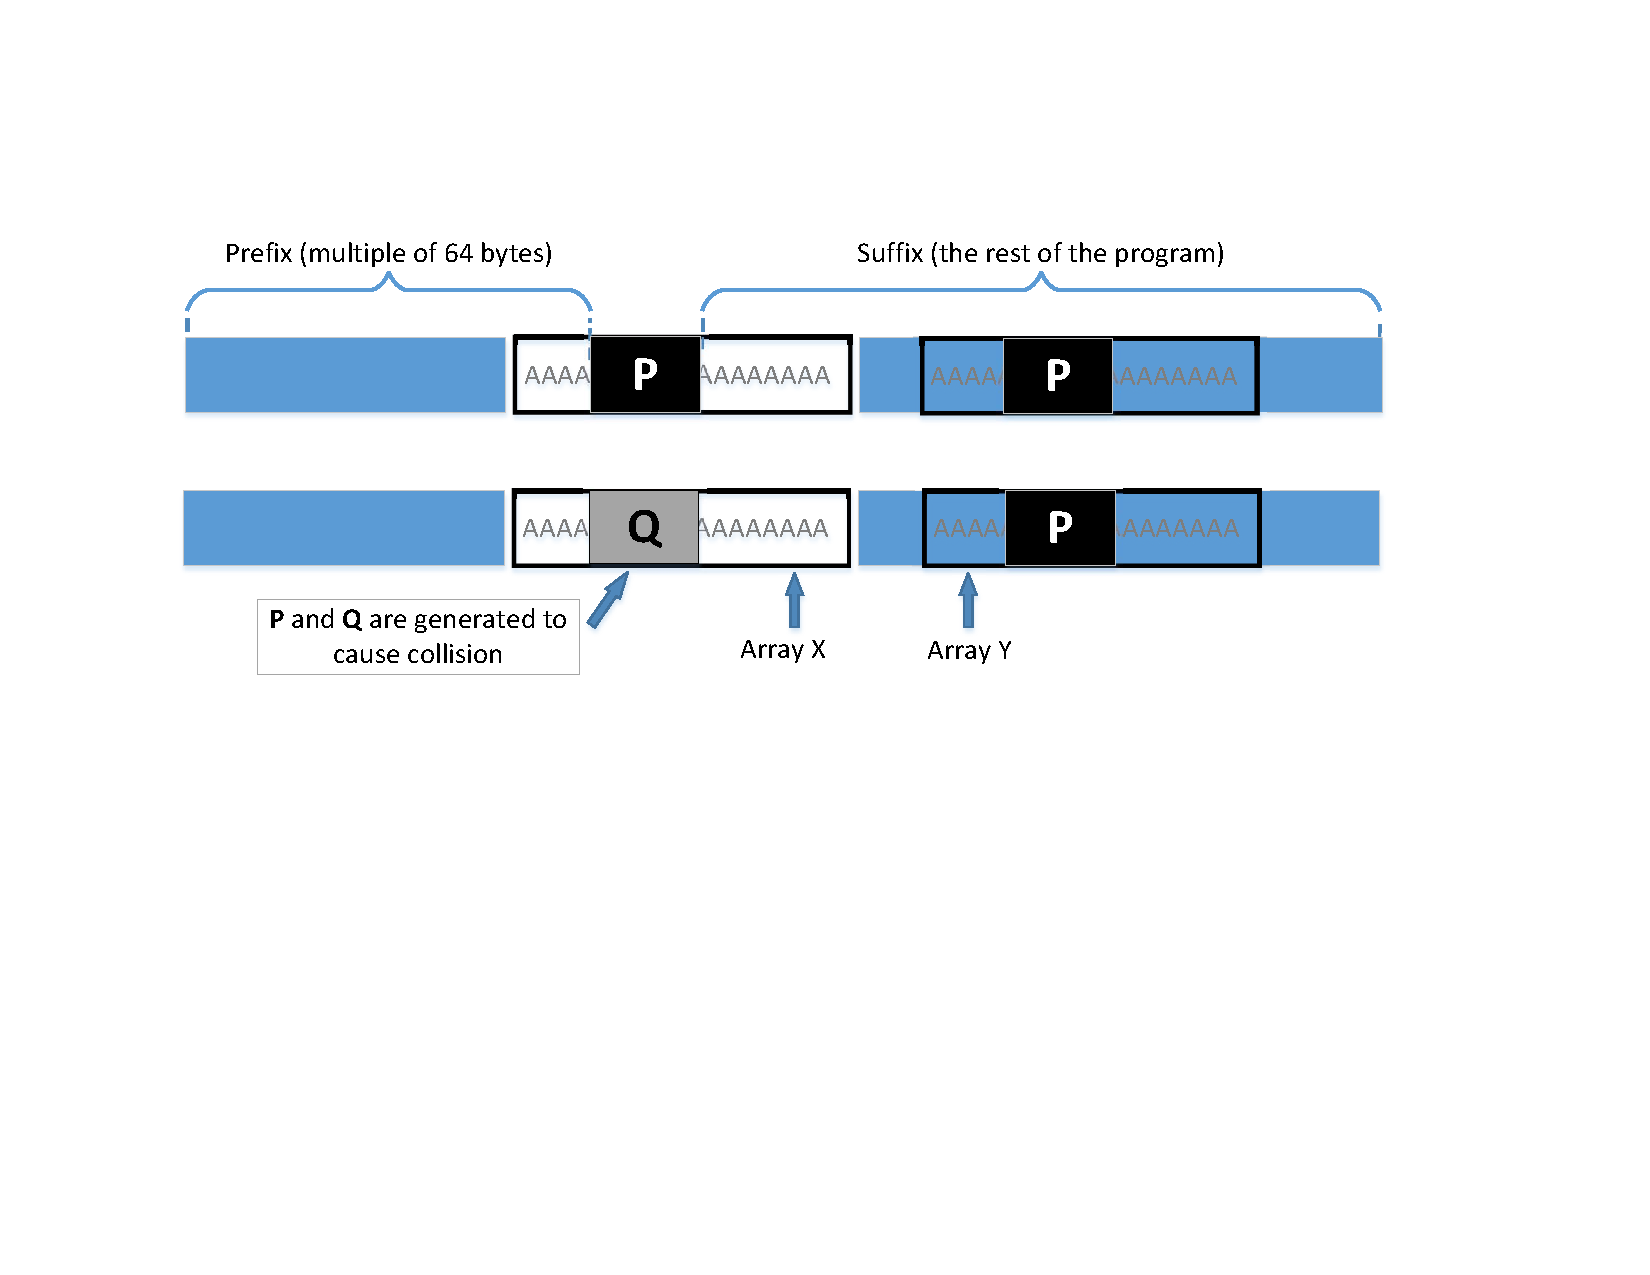
\includegraphics[width=0.9\textwidth]{\mdFigs/two_versions.pdf}
	\caption{一种生成两个行为不同但哈希冲突的程序的方法}
	\label{md5:fig:two_versions}
\end{figure}

从 \autoref{md5:fig:two_versions} 中,我们知道只要相应地生成 \texttt{P} 和
\texttt{Q},这两个二进制文件就具有相同的 MD5 哈希值。
在第一个版本中,使数组 X 和 Y 的内容相同,而在第二个版本中,使它们的内容不同。
因此,我们唯一需要更改的就是这两个数组的内容,而无需更改程序的逻辑。


%\paragraph{Questions.} After finishing this task, please answer the following questions:
%
%
%\begin{itemize}[label={--}]
%\item \textbf{Problem 5.} In Figure~\ref{md5:fig:two_versions}, can we place array \texttt{Y} in the prefix instead of
%in the suffix? Please explain.

%\item \textbf{Problem 6.} Given an existing program made by other people, can we use the
%\texttt{md5collgen} program to create  different program that has the same value as this
%existing one?  Please explain.
%\end{itemize}



% *******************************************
% SECTION
% *******************************************
\section{Submission}


%%%%%%%%%%%%%%%%%%%%%%%%%%%%%%%%%%%%%%%%

You need to submit a detailed lab report, with screenshots,
to describe what you have done and what you have observed.
You also need to provide explanation
to the observations that are interesting or surprising.
Please also list the important code snippets followed by
explanation. Simply attaching code without any explanation will not
receive credits.

%%%%%%%%%%%%%%%%%%%%%%%%%%%%%%%%%%%%%%%%


%%%%%%%%%%%%%%%%%%%%%%%%%%%%%%%%%%%%%%%%%%%%%%%%%%%%%%%%%%%%%%%%%%%%%%
\bibliographystyle{plain}
\def\baselinestretch{1}
\bibliography{BibMD5Lab}
%%%%%%%%%%%%%%%%%%%%%%%%%%%%%%%%%%%%%%%%%%%%%%%%%%%%%%%%%%%%%%%%%%%%%%


\end{document}
